% Include LaTeX packages
\documentclass[a4paper]{acmsiggraph}
\usepackage[a4paper, total={6.5in, 9in}]{geometry}
\usepackage{babel}
\usepackage{comment} % enables the use of multi-line comments (\ifx \fi)
\usepackage{enumitem}
\usepackage{amsmath,amsthm,amssymb}
\usepackage{listings}
\usepackage{graphicx}
\usepackage{etoolbox}
\usepackage{verbatim}

\usepackage[dvipsnames]{xcolor}
\usepackage{fancyvrb}
\usepackage{hyperref}
\usepackage{menukeys}
\usepackage{titlesec}
\usepackage[section]{placeins}
\usepackage{lipsum}

% Set additional LaTeX options
\setlength{\parskip}{.8mm}
\setcounter{MaxMatrixCols}{20}

\hypersetup{
	colorlinks=true,
	pdfauthor=A.~Mhamdi,
 	pdftitle=Template for Lab. assessment,
	pdfsubject=Lab. assessment to be submitted by students using this provided \LaTeX\ template,
	urlcolor=[rgb]{0.2,0.,0.8},
	anchorcolor={0.97,0,0.30},
	linkcolor=black,
	filecolor=[rgb]{0.97,0,0.30},
}

% Redefine \VerbatimInput
\RecustomVerbatimCommand{\VerbatimInput}{VerbatimInput}%
{fontsize=\footnotesize,
	%
	frame=lines, % top and bottom rule only
	framesep=2em, % separation between frame and text
	rulecolor=\color{Gray},
	%
	label=\fbox{\color{Black}\textbf{OUTPUT}},
	labelposition=topline,
	%
	commandchars=\|\(\), % escape character and argument delimiters for commands within the verbatim
	commentchar=* % comment character
}

% Set addditional formatting options
\titlespacing*{\section}{0pt}{5.5ex plus 1ex minus .2ex}{2ex}
\titlespacing*{\subsection}{0pt}{3ex}{2ex}
\setcounter{secnumdepth}{4}
\renewcommand\theparagraph{\thesubsubsection.\arabic{paragraph}}
\newcommand\subsubsubsection{\paragraph}

% Define a convenient norm symbol
\newcommand{\norm}[1]{\left\lVert#1\right\rVert}
\renewcommand{\vec}[1]{\mathbf{#1}}

% Define a macro for hiding answers
\newbool{hideanswers} \setbool{hideanswers}{false}
\newenvironment{answer}{}{}
\ifbool{hideanswers}{\AtBeginEnvironment{answer}{\comment} %
	\AtEndEnvironment{answer}{\endcomment}}{}

% Define text formatting for points and normals
\newcommand{\points}[1]{\hfill \normalfont{(\textit{#1pts})}}
\newcommand{\pointsin}[1]{\normalfont{(\textit{#1pts})}}

\usepackage{tikz}
\usetikzlibrary{shapes,decorations}
\usepackage{amsmath,amssymb}
\usepackage[]{nicefrac}

%%%%%%%%%%%%%%%%%%
\usepackage{pgfplots}
\pgfplotsset{compat=newest}
\pgfplotsset{plot coordinates/math parser=false}
\newlength\figureheight
\newlength\figurewidth
%%%%%%%%%%%%%%%%%%

\usepackage{fancyhdr}

\pagestyle{fancy}
\fancyhf{}
\fancyhead[L]{\bfseries\nouppercase\leftmark}
\fancyhead[R]{\thepage}

% Define title, author, and affiliation information
\title{<MODULE>\\ \LARGE {<LAB>}}
\author{\Large \begin{tabular}{ccc} <STUDENT 1> && <STUDENT 2> \\
\href{mailto:<EMAIL 1>}{<EMAIL 1>} && \href{mailto:<EMAIL 2>}{<EMAIL 2>} \\ & TERM : {\scshape <TERM>} &\\ \end{tabular} }

% Define box and box title style
\tikzstyle{mybox} = [draw=blue!40!red, fill=white, very thick,
rectangle, rounded corners, inner sep=10pt, inner ysep=20pt]
\tikzstyle{fancytitle} =[fill=blue!40!red, text=black]

% Definition of \maketitle
\makeatletter         
\def\@maketitle{
    \raggedleft\includegraphics[width=2cm]{images/logo-isetbz.jpg}
    \begin{center}
		{\Huge \bfseries \sffamily \@title }\\[4ex] 
		{\Large  \@author}\\[4ex] 
		\@date\\[8ex]
    \end{center}}
\makeatother

\usepackage{pifont} % http://ctan.org/pkg/pifont
\newcommand{\cmark}{\ding{51}}%
\newcommand{\xmark}{\ding{55}}%

\pdfauthor{A.~Mhamdi}

\begin{document}

\maketitle

\hrule
\setcounter{tocdepth}{2}
\tableofcontents
\vspace{0.25cm}
\hrule

\nocite{*}

\vspace{0.5cm}

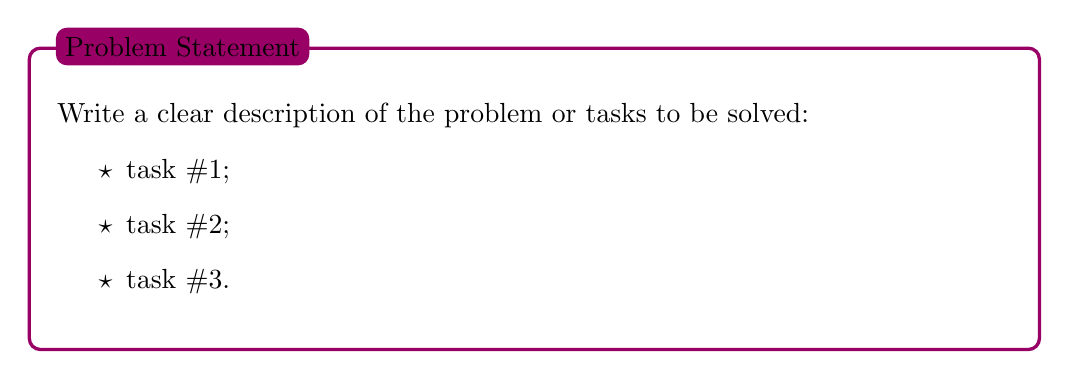
\begin{tikzpicture}
	\node [mybox] (box){%
		\begin{minipage}{\textwidth}
			Write a clear description of the problem or tasks to be solved:
			\begin{itemize}[label=$\star$]
				\item task \#1;
				\item task \#2;
                    \item task \#3.
			\end{itemize}
		\end{minipage}
	};
	\node[fancytitle, right=10pt, rounded corners] at (box.north west) {Problem Statement};
	\end{tikzpicture}%
 
\section{Introduction}
\lipsum[1]

Fig.~\ref{fig:isetbz} shows the logo of ISET Bizerte.

 \begin{figure}[!tbh]
 	\centering
 	\includegraphics[width=3cm]{./images/logo-isetbz.jpg}
 	\caption{Logo of ISET Bizerte.}
 	\label{fig:isetbz}
 \end{figure}

\section{Background Information}
\lipsum[1]

\begin{answer}
    \rule{\textwidth}{0.4pt}
    \textbf{Answers:}
    \begin{enumerate}[label=(\roman*)]
        \item Write your answer to question \#1 here.
        \item Write your answer to question \#2 here.
        \item Write your answer to question \#3 here.
        \item Write your answer to question \#4 here.
    \end{enumerate}
    \rule{\textwidth}{0.4pt}
\end{answer}

\section{Methodology \& Implementation Details}
\subsection{Approach}
\lipsum[2]

\subsection{Workflow and Pseudocode}
\lipsum[3]

\subsection{Results and Analysis}
\lipsum[4]

\section{Conclusion}
\lipsum[1]

%%% BIBLIOGRAPHY %%%
\bibliographystyle{apalike}
\bibliography{./biblio.bib}

\end{document} 
